\documentclass{article}
\usepackage[utf8]{inputenc}
\usepackage[english]{babel}
\usepackage{amsmath,amsfonts,amssymb,amsthm}
\usepackage{mathtools}
\usepackage{fancyhdr}
\usepackage{commath}
\usepackage[sc,osf]{mathpazo}
\usepackage{graphicx}
\usepackage{rotating}
\usepackage{float}
\usepackage{subcaption}
\restylefloat{table}
\usepackage{multicol}
\usepackage[dvipsnames]{xcolor}
\usepackage[colorinlistoftodos]{todonotes}
\usepackage{vmargin}  % Administrar márgenes
\setpapersize{A4} % Definir tamaño del papel
\setmargins{3cm} % Margen izquierdo
{1cm} % Margen superior
{15cm} % Área de impresión horizontal
{23.42cm} % Area de impresión vertical
{15mm} % Encabezado
{7mm} % Espacio entre el encabezado y el texto
{10pt} % Pie de página
{3mm} % Espacio entre el pie de página y el texto

\pagestyle{fancy}
\fancyhf{}
\rhead{

\includegraphics[width=4cm,height=1cm]{cropped-iitpal-at-prutor-logo.png}
}
\lhead{Circles | Class XI | Exemplar Problems}
\rfoot{}
\begin{document}
\section*{Practice Questions}
\paragraph{Q1.}Find the equation of the circle which passes through the points (20, 3),
(19, 8) and (2, -9). Find its centre and radius.
\begin{flushright}
Page-193
\end{flushright}

\paragraph{Q2.}The equation of the circle having centre (1, -2) and passing through the
point of intersection of the lines $3x + y = 14$ and $2x + 5y = 18$ is\
\begin{enumerate}
    \item $x^2 + y^2 - 2x + 4y - 20 = 0$
    \item $x^2 + y^2 - 2x - 4y - 20 = 0$
    \item $x^2 + y^2 + 2x - 4y - 20 = 0$
    \item $x^2 + y^2 + 2x + 4y - 20 = 0$
\end{enumerate}
\begin{flushright}
    Page-197, 202
\end{flushright}

\paragraph{Q3.}Find the equation of the circle which touches the both axes in first quadrant and
whose radius is a.
\begin{flushright}
    Page-202
\end{flushright}

\paragraph{Q4.}If a circle passes through the point (0, 0) (a, 0), (0, b) then find the coordinates of
its centre.
\begin{flushright}
    Page-202
\end{flushright}
\clearpage


\section*{Solution and Hints}
\paragraph{S1.}\
This is a simple application of class notes formulas. If one remebers the formulas using some trick, then it can be done easily just by putting values in formulas. We can solve 3 equations to get 3 unknowns of general form.\
By substitution of coordinates in the general equation of the  circle given by
$$x^2 + y^2 + 2gx + 2fy + c = 0$$, we have
\begin{align*}
    40g + 6f + c = - 409\\
    38g + 16 f + c = - 425\\
    4g - 18 f + c = - 85
\end{align*}
From these three equations, we get
g = - 7, f = - 3 and c = -111
Hence, the equation of the circle is
\begin{align*}
    x^2 + y^2 - 14x - 6y - 111 = 0\\
    \implies (x - 7)^2 + (y - 3)^2 = 132
\end{align*}
Therefore, the centre of the circle is (7, 3) and radius is 13.

\paragraph{S2.}\
Note that to get intersection point of two lines we just need to solve two linear equation problem.
\begin{align*}
    3x + y - 14 = 0\\
    2x + 5y - 18 = 0
\end{align*}
This gives us intersection point: $x=4, y=2$. Now radius of circle is:
\begin{align*}
    r^2&=(4-1)^2+(2+2)^2\\
    &=9+16=25
\end{align*}
We have radius = 5. Then $c$ in general form is,
\begin{align*}
    c&=g^2+f^2-r^2\\
    &=(-1)^2+(2)^2-25=-20
\end{align*} 
So general form is,
$$x^2 + y^2 - 2x + 4y - 20 = 0$$
Hence option (1) is right.

\paragraph{S3.}\
It can be done just by looking at the below picture,
% There is some problem in rendering this image
\begin{figure}[H]
    \centering
    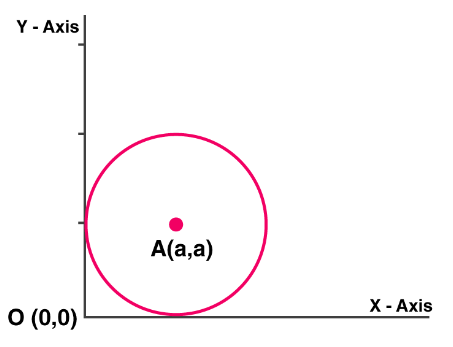
\includegraphics[scale=0.3]{l2_ps2-3.png}
    \caption{Circle with radius a}
\end{figure}
Now we can write equation of the center,
\begin{equation*}
    (x-a)^2+(y-a)^2=a^2
\end{equation*}.

\paragraph{S4.}\
This is also a simple application of class notes formulas, like que-1.
By substitution of coordinates in the general equation of the  circle given by
$$x^2 + y^2 + 2gx + 2fy + c = 0$$, we have
\begin{align*}
    c = 0\\
    a^2 + 2ga + c = 0\\
    b^2 + 2fb + c = 0
\end{align*}
From these three equations, we get center as
\begin{align*}
    -g&=\frac{a}{2}\\
    -f&=\frac{b}{2}
\end{align*}
And radius to be,
\begin{equation*}
    r^2=g^2+f^2-c=\frac{a^2+b^2}{4}
\end{equation*}
Hence, the equation of the circle is
\begin{align*}
     \left(x - \frac{a}{2}\right)^2 + \left(y - \frac{b}{2}\right)^2 = \frac{a^2+b^2}{4}
\end{align*}

\end{document}